\documentclass[aspectratio=169]{beamer}

\usepackage[T1]{fontenc}
\usepackage[utf8]{inputenc}
\usepackage{libertine}
\usepackage{xcolor}
\usepackage{tikz}
\usetikzlibrary{positioning,calc,shapes.geometric,backgrounds}
\usepackage{booktabs}
\usepackage{colortbl}
\usepackage{fontawesome5}

% ---------------------------------------------------------------------
% Palette
% ---------------------------------------------------------------------
\definecolor{dustyrose}{RGB}{199,123,132}
\definecolor{sage}{RGB}{131,158,140}
\definecolor{lavender}{RGB}{178,163,199}
\definecolor{cream}{RGB}{250,247,242}
\definecolor{charcoal}{RGB}{58,56,53}

\setbeamertemplate{navigation symbols}{}

\setbeamercolor{normal text}{fg=charcoal,bg=cream}
\setbeamercolor{structure}{fg=dustyrose}
\setbeamercolor{alerted text}{fg=sage}
\setbeamercolor{title}{fg=charcoal}
\setbeamercolor{author}{fg=charcoal}
\setbeamercolor{frametitle}{fg=charcoal,bg=cream}
\setbeamercolor{footline}{fg=charcoal,bg=cream}
\setbeamercolor{itemize item}{fg=dustyrose}
\setbeamercolor{itemize subitem}{fg=sage}
\setbeamercolor{enumerate item}{fg=dustyrose}
\setbeamercolor{block title}{fg=cream,bg=dustyrose}
\setbeamercolor{block body}{fg=charcoal,bg=dustyrose!8}
\setbeamercolor{caption name}{fg=sage}

\setbeamertemplate{itemize items}[circle]
\setbeamertemplate{enumerate items}[default]

\setbeamerfont{frametitle}{size=\Large,series=\bfseries}
\setbeamerfont{framesubtitle}{size=\normalsize,series=\itshape}

\setbeamertemplate{frametitle}{
  \vspace{0.15cm}
  \hspace{0.15cm}{\usebeamerfont{frametitle}\usebeamercolor[fg]{frametitle}\insertframetitle}\\[2pt]
  \hspace{0.15cm}{\color{sage}\rule{0.88\paperwidth}{0.6pt}}
}

\setbeamertemplate{footline}{%
  \begin{beamercolorbox}[wd=\paperwidth,ht=2.6ex,dp=1.3ex,leftskip=0.4cm,rightskip=0.4cm]{footline}
    {\color{charcoal!55}\scriptsize The Poetics of Ruin \hfill Naomi Prescott \hfill \insertframenumber\,/\,\inserttotalframenumber}
  \end{beamercolorbox}%
}

\newcommand{\yrtext}[1]{{\scriptsize\itshape\color{charcoal!65}#1}}

\newcommand{\sectiondivider}[2]{%
\begin{frame}[plain]
\begin{tikzpicture}[remember picture,overlay]
\fill[cream] (current page.south west) rectangle (current page.north east);
\fill[lavender!22] (current page.north west) rectangle ([shift={(0,-2.8cm)}]current page.north east);
\node[circle,fill=dustyrose!22,minimum size=2.6cm] at ([shift={(3.0cm,-3.2cm)}]current page.north west) {};
\node[circle,fill=sage!20,minimum size=1.5cm] at ([shift={(2.0cm,-4.9cm)}]current page.north west) {};
\node[circle,fill=lavender!25,minimum size=1.0cm] at ([shift={(-1.6cm,-2.0cm)}]current page.north east) {};
\node[align=center] at (current page.center) {%
  \begin{minipage}{0.72\paperwidth}
  \centering
  {\color{charcoal!75}\fontsize{11}{13}\selectfont\scshape #1}\\[10pt]
  {\color{dustyrose}\rule{3.2cm}{1pt}}\\[10pt]
  {\color{charcoal}\fontsize{28}{32}\selectfont\bfseries #2}
  \end{minipage}%
};
\end{tikzpicture}
\end{frame}%
}

\title{The Poetics of Ruin}
\author{Dr.\ Naomi Prescott}
\institute{Department of Comparative Literature, Meridian University}
\date{}

\begin{document}

% ---------------------------------------------------------------------
\begin{frame}[plain]
\begin{tikzpicture}[remember picture,overlay]
\fill[cream] (current page.south west) rectangle (current page.north east);
\fill[dustyrose!12] (current page.north west) rectangle ([shift={(0,-4.2cm)}]current page.north east);
\node[circle,fill=sage!18,minimum size=3.1cm] at ([shift={(-2.6cm,-5.1cm)}]current page.north east) {};
\node[circle,fill=lavender!25,minimum size=1.8cm] at ([shift={(-1.0cm,-6.7cm)}]current page.north east) {};
\node[circle,fill=dustyrose!16,minimum size=1.2cm] at ([shift={(2.6cm,-1.2cm)}]current page.south west) {};
\node at (current page.center) {%
\begin{minipage}{0.8\paperwidth}
\centering
{\color{dustyrose}\rule{4cm}{1pt}}\\[10pt]
{\color{charcoal}\fontsize{26}{30}\selectfont\bfseries The Poetics of Ruin}\\[5pt]
{\color{charcoal!80}\Large\itshape Memory, Nostalgia, and the Modern Novel}\\[20pt]
{\color{dustyrose}\rule{4cm}{1pt}}\\[18pt]
{\color{charcoal}\large Dr.\ Naomi Prescott}\\[3pt]
{\color{charcoal!70}\small Department of Comparative Literature \textbullet\ Meridian University}\\[10pt]
{\color{charcoal!58}\small HUM 342 \textbullet\ Autumn Lecture Series \textbullet\ 24 July 2026}
\end{minipage}%
};
\end{tikzpicture}
\end{frame}

% ---------------------------------------------------------------------
\begin{frame}[plain]
\begin{tikzpicture}[remember picture,overlay]
\fill[cream] (current page.south west) rectangle (current page.north east);
\node[circle,fill=sage!14,minimum size=2.2cm] at ([shift={(2.2cm,-2.0cm)}]current page.north west) {};
\node at (current page.center) {%
\begin{minipage}{0.74\paperwidth}
\centering
{\color{dustyrose}\fontsize{34}{34}\selectfont\faQuoteLeft}\\[14pt]
{\color{charcoal}\LARGE\itshape ``The house does not remember; it is we who furnish its silence with our own ruins.''}\\[16pt]
{\color{charcoal!70}\normalsize --- Ilse Kova\v{c}, \textit{The Unswept Room} (1962)}
\end{minipage}%
};
\end{tikzpicture}
\end{frame}

% ---------------------------------------------------------------------
\begin{frame}{Agenda}
\begin{columns}[T]
\begin{column}{0.5\textwidth}
\begin{itemize}
  \item[\textcolor{dustyrose}{I.}] Framing the Problem
  \begin{itemize}
    \item[\textcolor{sage}{--}] Why memory, why now
    \item[\textcolor{sage}{--}] A shared vocabulary
  \end{itemize}
  \item[\textcolor{dustyrose}{II.}] Ruins and Nostalgia
  \begin{itemize}
    \item[\textcolor{sage}{--}] The Romantic inheritance
    \item[\textcolor{sage}{--}] Three exemplary works
    \item[\textcolor{sage}{--}] Four literary moments
  \end{itemize}
\end{itemize}
\end{column}
\begin{column}{0.5\textwidth}
\begin{itemize}
  \item[\textcolor{dustyrose}{III.}] Case Studies
  \begin{itemize}
    \item[\textcolor{sage}{--}] \textit{The Unswept Room}
    \item[\textcolor{sage}{--}] \textit{Letters to the Drowned City}
    \item[\textcolor{sage}{--}] A synthesis
  \end{itemize}
  \item[\textcolor{dustyrose}{IV.}] Conclusions
  \begin{itemize}
    \item[\textcolor{sage}{--}] Key takeaways
    \item[\textcolor{sage}{--}] Further reading
  \end{itemize}
\end{itemize}
\end{column}
\end{columns}
\end{frame}

% ---------------------------------------------------------------------
\section{Framing the Problem}
\sectiondivider{Part One}{Framing the Problem}

% ---------------------------------------------------------------------
\begin{frame}{Why Memory, Why Now}
\begin{itemize}
  \item The modern novel is haunted less by what happened than by what remains of it: a room left unswept, a letter never posted, a name half-erased from a headstone.
  \item Since the mid-twentieth century, criticism has increasingly treated memory not as a theme among others but as the novel's proper subject --- its way of organizing time itself.
  \item Three pressures converge here: the collapse of stable national pasts after 1945, the rise of psychoanalytic models of the self, and a simple formal fact --- prose fiction is uniquely suited to representing consciousness recollecting itself.
  \item Our task this term is to read memory as \alert{form}, not merely content: how syntax, tense, and structure enact forgetting and recall.
\end{itemize}
\end{frame}

% ---------------------------------------------------------------------
\begin{frame}{Key Terms}
\renewcommand{\arraystretch}{1.35}
\begin{center}
\begin{tabular}{p{3.3cm} p{7.6cm}}
\rowcolor{dustyrose!15}
\textbf{Term} & \textbf{Working Definition} \\
\midrule
Nostalgia & A longing for a home that may never have existed as it is remembered. \\
\rowcolor{sage!10}
Ruin gaze & The aesthetic pleasure taken in decayed structures as sites of temporal reflection. \\
Involuntary memory & Recollection triggered by sensory accident rather than conscious will. \\
\rowcolor{sage!10}
Palimpsest & A text or place bearing visible traces of what it has overwritten. \\
\end{tabular}
\end{center}
\end{frame}

% ---------------------------------------------------------------------
\section{Ruins and Nostalgia}
\sectiondivider{Part Two}{Ruins and Nostalgia}

% ---------------------------------------------------------------------
\begin{frame}{The Romantic Ruin}
\begin{itemize}
  \item Before the novel claimed it, the ruin belonged to poetry and to the picturesque garden: a fragment arranged to provoke feeling rather than to record fact.
  \item The Romantic ruin is never simply decayed matter --- it is decay staged for a viewer, evidence that time is visible and that the viewer survives it.
  \item Nineteenth-century fiction inherits this staging but complicates it: the ruined house in the domestic novel is inhabited, still paying its taxes, still expected to hold a family together.
  \item Margarethe Voss names this the \textit{lived ruin} --- a structure that has not yet been granted the dignity of collapse, and must instead go on being lived in.
\end{itemize}
\end{frame}

% ---------------------------------------------------------------------
\begin{frame}{Three Exemplary Works}
\renewcommand{\arraystretch}{1.3}
\begin{center}
\begin{tabular}{p{3.4cm} p{2.6cm} c p{3.6cm}}
\rowcolor{dustyrose!15}
\textbf{Work} & \textbf{Author} & \textbf{Year} & \textbf{Central Motif} \\
\midrule
\textit{The Unswept Room} & Ilse Kova\v{c} & 1962 & the abandoned family house \\
\rowcolor{sage!10}
\textit{Letters to the Drowned City} & Tomasz Aldana & 1978 & a flooded harbor town \\
\textit{Ash and Almanac} & Margarethe Voss & 1991 & the burned family archive \\
\end{tabular}
\end{center}
\vspace{8pt}
\small\color{charcoal!70} Each work substitutes a physical remainder --- house, harbor, archive --- for the memory it can no longer trust the narrator to supply directly.
\end{frame}

% ---------------------------------------------------------------------
\begin{frame}{Four Moments in the Literature of Memory}
\begin{center}
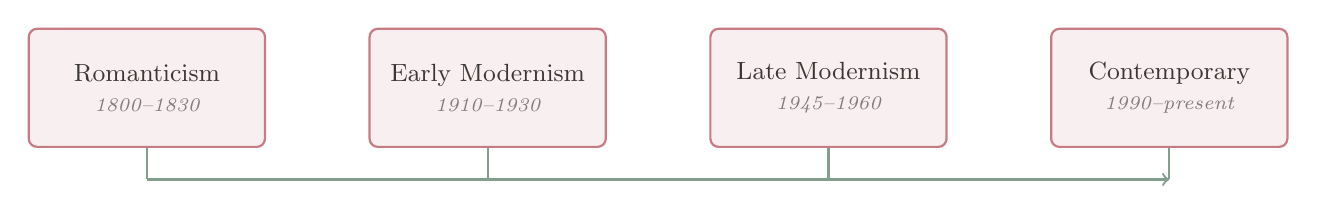
\begin{tikzpicture}[
  node distance=1.1cm and 1.3cm,
  period/.style={rectangle,rounded corners=3pt,draw=dustyrose,thick,
    fill=dustyrose!12,minimum width=3.0cm,minimum height=1.5cm,
    align=center,font=\small\selectfont,text=charcoal}
]
\node[period] (n1) {Romanticism\\\yrtext{1800--1830}};
\node[period,right=of n1] (n2) {Early Modernism\\\yrtext{1910--1930}};
\node[period,right=of n2] (n3) {Late Modernism\\\yrtext{1945--1960}};
\node[period,right=of n3] (n4) {Contemporary\\\yrtext{1990--present}};
\draw[sage,thick,->] ($(n1.south)+(0,-0.4)$) -- ($(n4.south)+(0,-0.4)$);
\draw[sage,thick] (n1.south) -- ($(n1.south)+(0,-0.4)$);
\draw[sage,thick] (n2.south) -- ($(n2.south)+(0,-0.4)$);
\draw[sage,thick] (n3.south) -- ($(n3.south)+(0,-0.4)$);
\draw[sage,thick] (n4.south) -- ($(n4.south)+(0,-0.4)$);
\end{tikzpicture}
\end{center}
\vspace{6pt}
\begin{itemize}
  \small
  \item The picturesque ruin gives way to the psychological interior, then to the archival fragment, then to memory understood as data --- recorded, searchable, and no less unreliable.
  \item Our case studies this term sit at the hinge between the second and third moments.
\end{itemize}
\end{frame}

% ---------------------------------------------------------------------
\section{Case Studies}
\sectiondivider{Part Three}{Case Studies}

% ---------------------------------------------------------------------
\begin{frame}{Case Study: \textit{The Unswept Room} (1962)}
\begin{itemize}
  \item Ilse Kova\v{c}'s narrator, Ana Sever, returns to her late mother's house and refuses --- for the length of the novel --- to clean a single room.
  \item The house is narrated in the present tense throughout, even as its contents are unmistakably historical; Kova\v{c} uses tense itself to argue that the past is never fully past.
  \item Dust becomes a formal device: each undisturbed surface marks a memory the narrator has not yet permitted herself to revisit.
  \item By the final chapter, sweeping the room is not an act of closure but of erasure --- and the novel treats this as a loss, not a triumph.
\end{itemize}
\end{frame}

% ---------------------------------------------------------------------
\begin{frame}{Case Study: \textit{Letters to the Drowned City} (1978)}
\begin{itemize}
  \item Tomasz Aldana's epistolary novel is composed entirely of letters written by a harbor engineer to a city that has already been submerged by a dam project.
  \item Because the addressee cannot reply, the letters accumulate without correction --- each one revising the last, so the reader assembles memory as a series of retractions rather than facts.
  \item Aldana's prose style shifts from precise, technical description early on to increasingly figurative language as the engineer's certainty about what actually happened erodes.
  \item Critics have read the flooded city as a rebuke to the ruin gaze: there is no picturesque wreck here to admire, only water with nothing left above it to survive.
\end{itemize}
\end{frame}

% ---------------------------------------------------------------------
\begin{frame}{A Synthesis}
\begin{itemize}
  \item Both novels displace memory onto an object --- a room, a drowned city --- that the narrator can describe but not fully master.
  \item Both resist a single authoritative timeline: Kova\v{c} through tense, Aldana through the accumulating, self-revising letter form.
  \item Where they diverge is instructive: Kova\v{c}'s ruin can still be swept, still argued with; Aldana's has already passed beyond any possibility of repair.
  \item Read together, they trace the arc from the \textit{lived ruin} to what Voss calls the \textit{irrecoverable} --- the point past which nostalgia has nothing left to reach for.
\end{itemize}
\end{frame}

% ---------------------------------------------------------------------
\section{Conclusions}
\sectiondivider{Part Four}{Conclusions}

% ---------------------------------------------------------------------
\begin{frame}{Key Takeaways}
\begin{enumerate}
  \item Memory in the modern novel is a formal problem before it is a thematic one --- attend to tense, structure, and narrating position.
  \item The ruin is never neutral scenery; it is always staged for someone, even when that someone is the narrator alone.
  \item Involuntary memory and the deliberate archive are not opposites but two ends of a single spectrum of control.
  \item The most instructive comparisons often come from works that treat the same motif --- the house, the drowned town --- with opposite formal strategies.
\end{enumerate}
\end{frame}

% ---------------------------------------------------------------------
\begin{frame}{Further Reading}
{\color{dustyrose}\faBook\ \textbf{Primary Works}}
\begin{itemize}
  \item Kova\v{c}, I. (1962). \textit{The Unswept Room}. Meridian University Press.
  \item Aldana, T. (1978). \textit{Letters to the Drowned City}. Nexa Editions.
  \item Voss, M. (1991). \textit{Ash and Almanac}. Vertex Academic.
\end{itemize}
\vspace{6pt}
{\color{sage}\faBook\ \textbf{Secondary Criticism}}
\begin{itemize}
  \item Voss, M. (1998). \textit{Ruins and Recollection: Essays on the Modern Elegy}. Meridian University Press.
  \item Aldana Jr., R. (2004). \textit{Water Memory: Reading the Flooded Text}. Nexa Editions.
  \item Kova\v{c}, I. \& Ferro, D. (2011). \textit{Domestic Ruins: The House as Archive}. Vertex Academic.
\end{itemize}
\end{frame}

% ---------------------------------------------------------------------
\begin{frame}[plain]
\begin{tikzpicture}[remember picture,overlay]
\fill[cream] (current page.south west) rectangle (current page.north east);
\fill[dustyrose!10] (current page.north west) rectangle ([shift={(0,-3.2cm)}]current page.north east);
\node[circle,fill=lavender!22,minimum size=2.4cm] at ([shift={(-2.2cm,-3.4cm)}]current page.north east) {};
\node[circle,fill=sage!18,minimum size=1.3cm] at ([shift={(2.4cm,-1.6cm)}]current page.south west) {};
\node at (current page.center) {%
\begin{minipage}{0.72\paperwidth}
\centering
{\color{charcoal}\fontsize{28}{30}\selectfont\bfseries Thank You}\\[8pt]
{\color{charcoal!75}\large\itshape Questions and discussion welcome}\\[22pt]
{\color{dustyrose}\rule{3.5cm}{1pt}}\\[16pt]
{\color{charcoal}\faEnvelope\ n.prescott@meridian.edu}\\[6pt]
{\color{charcoal}\faGlobe\ meridian.edu/complit/prescott}
\end{minipage}%
};
\end{tikzpicture}
\end{frame}

\end{document}
